\documentclass[a4paper,12pt]{article}
\usepackage[utf8]{inputenc}

\usepackage{fancyhdr} 
\usepackage[]{cite}
\usepackage{lastpage} 
\usepackage{extramarks} 
\usepackage{graphicx,color}
\usepackage{anysize}
\usepackage{amsmath}
\usepackage{natbib}
\usepackage{caption}
\usepackage{float}
\usepackage{url}
\usepackage{listings}
\usepackage[svgnames]{xcolor}
\usepackage[colorlinks=true, allcolors=black]{hyperref}
\usepackage[small]{titlesec}
\usepackage[version=4]{mhchem}
\usepackage{linegoal}


\textwidth=6.5in
\linespread{1.0} % Line spacing
\renewcommand{\familydefault}{\sfdefault}

% \titleformat{\section}
% {\normalfont\bfseries}
% {\thesection.}{0.75em}{}

\titlespacing{\section}{0pt}{0pt}{0pt}

%% includescalefigure:
%% \includescalefigure{label}{short caption}{long caption}{scale}{filename}
%% - includes a figure with a given label, a short caption for the table of contents and a longer caption that describes the figure in some detail and a scale factor 'scale'
\newcommand{\includescalefigure}[5]{
\begin{figure}[H]
\centering
\includegraphics[width=#4\linewidth]{#5}
\captionsetup{width=.8\linewidth} 
\caption[#2]{#3}
\label{#1}
\end{figure}
}

%% includefigure:
%% \includefigure{label}{short caption}{long caption}{filename}
%% - includes a figure with a given label, a short caption for the table of contents and a longer caption that describes the figure in some detail
\newcommand{\includefigure}[4]{
\begin{figure}[H]
\centering
\includegraphics{#4}
\captionsetup{width=.8\linewidth} 
\caption[#2]{#3}
\label{#1}
\end{figure}
}

%%------------------------------------------------
%% Parameters
%%------------------------------------------------
% Set up the header and footer
\pagestyle{fancy}
\lhead{\authorName} % Top left header
\chead{\moduleCode\ - \assignmentTitle} % Top center header
\rhead{\firstxmark} % Top right header
\lfoot{\lastxmark} % Bottom left footer
\cfoot{} % Bottom center footer
\rfoot{Page\ \thepage\ of\ \pageref{LastPage}} % Bottom right footer
\renewcommand\headrulewidth{0.4pt} % Size of the header rule
\renewcommand\footrulewidth{0.4pt} % Size of the footer rule

\setlength\parindent{0pt} % Removes all indentation from paragraphs
\newcommand{\assignmentTitle}{Table Tennis Assignment}
\newcommand{\moduleCode}{CSU44053} 
\newcommand{\moduleName}{Computer Vision} 
\newcommand{\authorName}{Liam Junkermann} 
\newcommand{\authorID}{19300141}
\newcommand{\reportDate}{\today}
% \renewcommand{\abstractname}{Introduction}

\title{
    \vspace{-1in}
    \begin{figure}[!ht]
    \flushleft
    
\includegraphics[width=0.4\linewidth]{Trinity_RGB_transparent_main.png}
    \end{figure}
    \vspace{-0.5cm}
    \hrulefill \\
    \vspace{1cm}
    \textmd{\textbf{\moduleCode\ \moduleName}}\\
    \textmd{\textbf{\assignmentTitle}}\\
    {
        \large
        \textmd{\authorName\ - \authorID}\\
        \textmd{\reportDate}\\
    }
    \vspace{0.5cm}
    \hrulefill \\
}
\date{}
\author{}
\begin{document}

\maketitle
\tableofcontents

\section{Finding Balls}
\subsection{Theory}
The balls are the easiest part of this assignment. There are three main ways to identify the table tennis balls.

\begin{description}
    \item[Colour-based Segmentation] This method uses the known colour value of the ball to determine where the ball is. This solution is quite quick and computationally cheap, however, it is susceptible to changes in light. It also requires the system to know the exact colour of a ball to work.
    \item[Contour Detection] Contour detection can be used to determine objects that might be table tennis balls. The final check for if a table tennis ball is present is to test circularity. Regardless of the angle at which a given image is taken, a table tennis ball will present as circular, allowing circularity to be used to determine which ball is the table tennis ball.  This method may be sensitive to noise but it is a good option. Additionally, dialling in the threshold value is difficult. Depending on lighting the ball may be only partially contoured, the text on the ball can also cause issues.
    \item[Edge Detection] Edge detection can be used to highlight contours and boundaries in an image. As the ball will generally contrast against the background, something which people need in order to play table tennis, it is safe to assume edge detection will perform well due to the changes in colour between the ball and the background. 
\end{description}

\subsection{Results \& Illustrations}
Contour detection and edge detection were tested to identify the balls. Both implementations used the same initial preprocessing. Images were converted to grayscale and a Guassian Blur was applied. The blur was applied to reduce noise in the converted images, doing much of the work to reduce false positives due to glare or reflections in the photographs.

Contour detection did not work as well as edge detection, issues included unideal lighting conditions and in one case the text on the ball. Contour detection also missed the orange balls entirely, only highlighting the nearly white portions of the ball.  In most cases, the contour detection failed to highlight the entire ball. The contouring initially produced a binary image which contained many more features, such as bright spots on the table, lines on the table, and in some cases the bright spots on the handle of the paddle. A minimum circularity test was added in order to rule out any classified features which could not be balls. The test did not look for entirely circular regions because of the aforementioned discrepancies due to inconsistent lighting conditions. 

Examples of unsuccessful contour detection can be found below in ~\autoref{fig:failed-contour}.
Examples of (mostly) successful contour detection can be found below in~\autoref{fig:success-contour}.

\begin{figure}[H]
    \centering
    \imageinners{fig:balls1-contour}{Ball Detection - Balls1}{A mostly successful detection of a ball: Balls1}{results/balls1-contourdetection.png}
    \hfill
    \imageinners{balls2-contour}{Ball Detection - Balls2}{Partial detection - Text error: Balls2}{results/balls2-contourdetection.png}
    \hfill
    \imageinners{balls6-contour}{Ball Detection - Balls6}{A successful detection of a ball: Balls6}{results/balls6-contourdetection.png}
    \caption{(Semi) Successful Contour Detections}
    \label{fig:success-contour}
\end{figure}

\begin{figure}[H]
    \centering
        \imageinners{balls8-contour}{Ball Detection - Balls8}{Unsuccessful ball detection (and misclassification): Balls8}{results/balls8-contourdetection.png}
    \hfill
        \imageinners{balls9-contour}{Failed ball detection - Balls9}{Entirely failed ball detection: Balls9}{results/balls9-contourdetection.png}
    \caption{Unsuccessful or Failed Contour Detection}
    \label{fig:failed-contour}
\end{figure}

Edge detection, using Hough for Circles, proved far more effective, especially with varying ball colours and lighting conditions. Using Hough for Circles is especially suited for this application because regardless of the angle at which the photo of the table tennis ball is taken, it will be projected as a circle. One issue was tuning the parameters to correctly identify balls of varying sizes across multiple images, but this step was relatively straightforward as the maximum size of a ball was still quite small. Hough results can be found in~\autoref{fig:hough-circles} and compared with the results from Contouring (\ref{fig:success-contour}, \ref{fig:failed-contour}).

\begin{figure}[H]
    \centering
    \imageinners{balls2-hough}{Ball Detection - Balls2}{Ball detection with Hough for Circles: Balls2}{results/balls2-hough.png}
    \imageinners{balls6-hough}{Ball Detection - Balls6}{Ball detection with Hough for Circles: Balls8}{results/balls6-hough.png}
    \imageinners{balls1-hough}{Ball Detection - Balls1}{Ball detection with Hough for Circles: Balls1}{results/balls1-hough.png}
    \imageinners{balls8-hough}{Ball Detection - Balls8}{Ball detection with Hough for Circles: Balls6}{results/balls8-hough.png}
    \imageinners{balls9-hough}{Ball Detection - Balls9}{Ball detection with Hough for Circles: Balls9}{results/balls9-hough.png}
    \caption{Hough for Circles Results}
    \label{fig:hough-circles}
\end{figure}

\subsection{Analysis}
It is clear Hough for circles was more effective for identifying table tennis balls. It was more resilient to changes in lighting conditions and colour than standard contour detection. As a result of using edge detection, it could separate the ball from the background, even when other objects in the background, such as the table tennis paddle, had similar values when converted to grayscale. Hough for Circles is therefore the chosen way to more consistently determine where the balls are.
\section{Finding tables}
\subsection{Theory}
Detecting tables was much tougher and I was not able to find the correct process to find the tables.
\section{Analysing play in video}
\subsection{Theory}
The video analysis is built more specifically for the video provided. The ball in the video never changes and lighting in the video is pretty good. We are able to convert each frame into HSL colour space and highlighting light and nearly white objects based on a range. This is then able to generate a mask with the ball, and some other lines or artifacts from the players. A grayscale image of each frame is then compared with the frame before it to find any changes, this difference is then thresholded to allow us to combine the HSV mask with the difference mask to find just the ball. Next, the position and the direction of travel of the ball are taken into account. The position is determined from the contours of the mask binary image produced from the previously mentioned steps. This position is then added to an array so that the direction of the ball can be considered. Any change in direction suggests how the ball as bounced, if a ball goes down and up it has bounced off the table, if the ball bounces right to left Player 1 has hit the ball, if the ball bounces left to right, player 2 has hit the ball. A bounding box around the net has been created to handle hits to the net. The bounding box does not include the full net because this may trigger false positives when the ball flies over the far side of the net. 
\subsection{Results \& Illustrations}
See below the video and data streaming.
\begin{figure}[H]
    \centering
    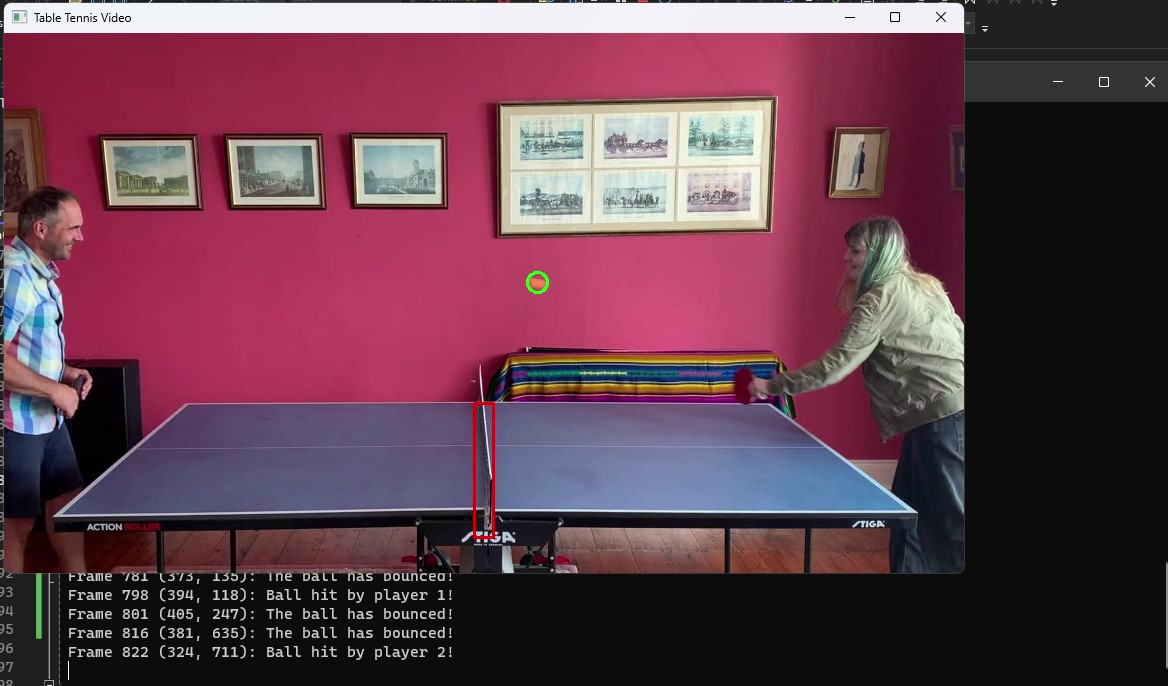
\includegraphics[width=0.75\textwidth]{results/frame.jpg}
    \caption{\href{https://youtu.be/y1nezl333-0}{Run through of Video Analysis}\href{https://youtu.be/y1nezl333-0}{https://youtu.be/y1nezl333-0}}
    \label{fig:vid-anyl}
\end{figure}

\subsection{Analysis}
There are some issues when a player first serves the ball. Due to the unexpected change in direction, hits are recorded sooner than they take place. Given more time, some more logic could be added to more accurately determine the hits off the net.

\end{document}